\textbf{Dilated Convolutions:} Maxpooling helps the network learn the global context of input feature maps but loses spatial resolution. Dilated convolutions allow for larger filters without adding additional parameters.  You can read more on Dilated convolutions \href{https://towardsdatascience.com/review-dilated-convolution-semantic-segmentation-9d5a5bd768f5}{here}. Consider the same input feature map used for question 1. Also consider the same filters provided for question 1. Fill in the values below after dilated convolution (with dilation factor 2) between the input feature map and the filters. (2 pts)

\begin{figure}[H]
	\centering
	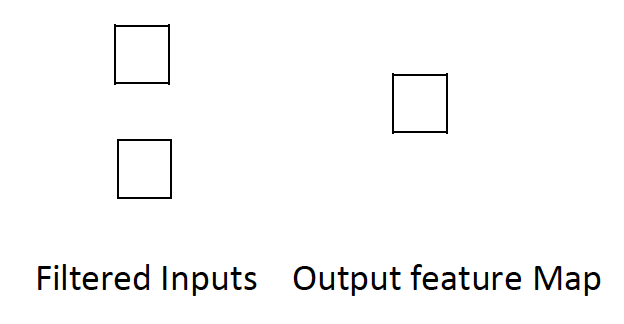
\includegraphics[width=.3\linewidth]{images/dilatedconv.png}
\end{figure}

\begin{tcolorbox}[title=Solution]
\end{tcolorbox}
